\newpage

\section{Rozpraszanie ramanowskie}
\subsection{Czym jest spektroskopia ramanowska?}
Spektroskopia ramanowska jest istotną metodą badania widm rotacyjnych i oscylacyjnych cząsteczek. Światło rozproszone ramanowsko ma inne częstości niż światło padające. Obserwujemy przesunięcie linii zarówno w stronę większych jak i mniejszych częstości, a tym samym większych i mniejszych energii. Kilka cech tej spektroskopii jest niezwykle ważnych. Jedną z nich jest możliwość użycia monochromatycznego źródła światła z zakresu widzialnego do otrzymania widma ramanowskiego. Można lepiej operować takim światłem w warunkach eksperymentalnych niż światłem podczerwonym lub mikrofalami. Niektóre dwuatomowe cząsteczki jak $\mathbf{H_{2}}$ czy $\mathbf{O_{2}}$ nie posiadają momentu dipolowego i dlatego nie są aktywne w podczerwieni, a ich widma mogą być obserwowane właśnie w spektroskopii ramanowskiej. Zatem np. pod tym względem spektroskopia ramanowska jest dopełnieniem spektroskopii w podczerwieni i odwrotnie. Poza tym spektroskopia ramanowska umożliwia badanie drgań cząsteczek, które zmieniając swoje położenie, wykonują np. ruchy obrotowe, co z kolei powoduje zmianę ich ukierunkowania względem padającego promieniowania. Objawia się to zmianą polaryzacji cząsteczki w stosunku do światła padającego. Ponadto rozpraszanie ramanowskie, podobnie jak spektroskopia w podczerwieni, dostarcza informacji o budowie cząsteczki, wiązaniach międzyatomowych, które ją tworzą, a także o ich polaryzowalności. Pozwala to w niektórych przypadkach przewidzieć reaktywność chemiczną i przebieg reakcji chemicznych.

Rozproszone ramanowsko fotony mogą służyć do identyfikacji rożnych rodzajów gazów. Reguły wyboru dla przejść ramanowskich są inne niż dla przejść w podczerwieni. Wszystkie dwuatomowe gazy są niewidoczne w podczerwieni ($\mathbf{O_{2}}$, $\mathbf{N_{2}}$, $\mathbf{H_{2}}$, $\mathbf{Cl_{2}}$), natomiast w widmie ramanowskim są widoczne. Dodatkową zaletą spektroskopii ramanowskiej jest to że można identyfikować składniki mieszaniny gazów. Z tego względu możliwe jest zastosowanie spektroskopii ramanowskiej przy produkcji paliwa gazowego w elektrowniach naturalnych lub biogazowych, w których monitorowanie obecności takich składników jak $\mathbf{CH_{4}}$, $\mathbf{CO_{2}}$, $\mathbf{O_{2}}$, $\mathbf{N_{2}}$ i $\mathbf{H_{2}}$ jest istotne. Dodatkową zaletą przy monitorowaniu tych substancji gazowych jest fakt, że obecność cząsteczek wody nie zaburza pomiaru ramanowskiego. Wykonywanie pomiarów ramanowskich i ich analiza może odbywać się na bieżąco w czasie procesu produkcyjnego. Dalszą zaletą pomiarów ramanowskich dla substancji gazowych jest możliwość rejestrowania wysokich stężeń tych gazów, ponieważ nie występuję efekt nasycenia. Objętość próbki użytej do badań w spektroskopii ramanowskiej może być bardzo mała, z tego względu możliwy jest pomiar ramanowski w mikroreaktorach używanych w chemii kombinatorycznej. Główną wadą spektroskopii ramanowskiej jest fakt, że proces rozpraszania ramanowskiego jest z reguły mało efektywny, co oznacza, że może wstępować problem w uzyskaniu akceptowalnej czułości. Większość spektrometrów ramanowskich jest przeznaczona do identyfikacji materiałów w stanie stałym lub płynnym, gdzie wyższa gęstość materiału znacząco zwiększa sygnał [7][9][13].

\subsection{Opis matematyczny}
Jeżeli światło o natężeniu 
\begin{equation}
	E = E_{m}\cos (2\pi f_{p}t)
\end{equation}
\begin{itemize}
	\item[-]{$E$ - natężenie padającego światła};
	\item[-]{$E_{m}$ - wartość maksymalna natężenia};
	\item[-]{$f_{p}$ - częstotliwość promieniowania padającego}.
\end{itemize}
pada na cząsteczkę, to wystąpi oddziaływanie pomiędzy wektorem $\overrightarrow{E}$, a elektronowymi powłokami atomów tworzących cząsteczkę.
Elektrony w cząsteczkach wykazują polaryzowalność $\alpha$, czyli zdolność przemieszczania
się pod wpływem pola elektrycznego. W wyniku takiego przemieszczenia jest indukowany w cząsteczce moment dipolowy.
\begin{equation}
	p_{i} = \alpha E = E_{m}\cos (2\pi f_{p}t)
\end{equation}
Wyindukowany moment dipolowy oscyluje z częstotliwością $f_{p}$ w skutek tego następuje emisja promieniowania o tej samej częstotliwości. Proces ten nosi nazwę \textit{rozpraszania Rayleigha}.

Jeśli dodatkowo uwzględnimy że cząsteczka wykonuje drgania z częstotliwością $f_{osc}$, to jej wychylenie z położenia równowagi można opisać wzorem, gdzie:
\begin{equation}
	r - r_{0} = r_{m}\cos (2\pi f_{osc}t)
\end{equation}
\begin{itemize}
	\item[-]{$r_{0}$ - położenie równowagi};
	\item[-]{$r_{m}$ - maksymalne wychylenie};
	\item[-]{$f_{osc}$ - częstotliwość drgań cząsteczki}.
\end{itemize}
Polaryzowalność cząsteczki zmienia się wraz ze zmianą $r$. Stąd może być przedstawiona w postaci szeregu potęgowego:
\begin{equation}
	\alpha(r) = \alpha(r_{0}) + \frac{d\alpha}{dr}(r - r_{0}) + 
	\frac{d^{2}\alpha}{dr^{2}}(r - r_{0})^{2} + ... +
	\frac{d^{n}\alpha}{dr^{n}}(r - r_{0})^{n}
\end{equation}
W dalszych przekształceniach nie będziemy uwzględniać wyrazów wyższych rzędów niż pierwszy. 

Uwzględniając wzory (1),(2),(3) możemy przedstawić moment dipolowy cząsteczki w następujący sposób:
\begin{equation}
	p(t) = \alpha E = 
	\left\{ 
		\alpha(r_{0}) + \frac{d\alpha}{dr}r_{m}\cos (2\pi f_{osc}t) 
	\right\}
	E_{m}\cos (2\pi f_{p}t)
\end{equation}
Możemy przekształcić powyższe równanie stosując wzór na iloczyn cosinusów:
\begin{equation}
	p(t) = \alpha(r_{0})E_{m}\cos (2\pi f_{p}t) + \frac{d\alpha}{dr}E_{m}r_{m}
	\left\{
		\cos (2\pi (f_{p} + f_{osc})t) + \cos (2\pi (f_{p} - f_{osc})t)
	 \right\}
\end{equation}
Ponieważ argumenty funkcji $\cos$ zawierają częstotliwości $f = f_{p} \pm f_{osc}$, dla tego będziemy je obserwować w widmie światła
rozproszonego. Wielkość przesunięcia ramanowskiego zależy od częstości drgań własnych cząsteczki i dla tego jest cechą charakterystyczną danej cząsteczki. Linie widma, które przesunięte są w stronę mniejszych energii, tworzą tzw. pasmo stokesowskie, a te przesunięte w stronę większych energii – pasmo antystokesowskie.
\begin{figure}[H]
	\begin{center}
		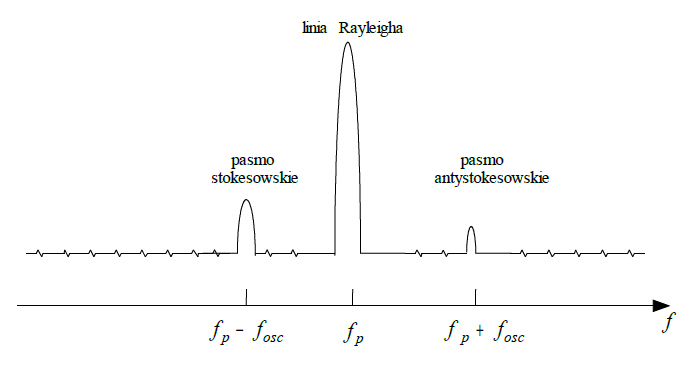
\includegraphics[width=1\linewidth]{Rozpraszanie-Ramanowskie/Schemat-widma-Ramanowskiego.png}
		\caption{Różne obszary widma ramanowskiego [10].}
	\end{center}
\end{figure}

\subsection{Rodzaje pasm obserwowanych w widmie ramanowskim}
W pomiarze widma ramanowskiego możemy zaobserwować trzy rodzaje pasm:
\begin{itemize}
	\item[-]{Pasmo Rayleigha};
	\item[-]{Pasmo stokesowskie};
	\item[-]{Pasmo antystokesowskie}.
\end{itemize}

\textbf{Pasmo Rayleigha} - powstające na skutek rozpraszania fotonów promieniowania padającego o częstości $\nu_{0}$, nie pasujących do poziomów energetycznych cząsteczki. Po oddziaływaniu fotonu z cząsteczką, wraca ona na ten sam poziom energetyczny.

\textbf{Pasmo stokesowskie} - gdy cząsteczka po oddziaływaniu z promieniowaniem ostatecznie przechodzi na wyższy poziom oscylacyjny. Wtedy foton rozproszony ma energię mniejszą w stosunku do fotonu padającego o różnicę energii poziomów oscylacyjnych $h\nu$.

\textbf{Pasma antystokesowskie} - jeśli przed oddziaływaniem z promieniowaniem molekuła znajduje się na wyższym poziomie oscylacyjnym, i wskutek oddziaływania z promieniowaniem przechodzi na poziom podstawowy oscylacyjny. Wtedy energia fotonu rozproszonego jest większa od energii fotonu padającego o różnicę energii poziomów oscylacyjnych $h\nu$. Pasmo antystokesowskie pojawia się w widmie Ramana po przeciwnej stronie co pasmo stokesowskie w stosunku do pasma Rayleigha. Pasmo to ma zwykle niższą intensywność niż pasma stokesowskie.
\begin{figure}[H]
	\begin{center}
		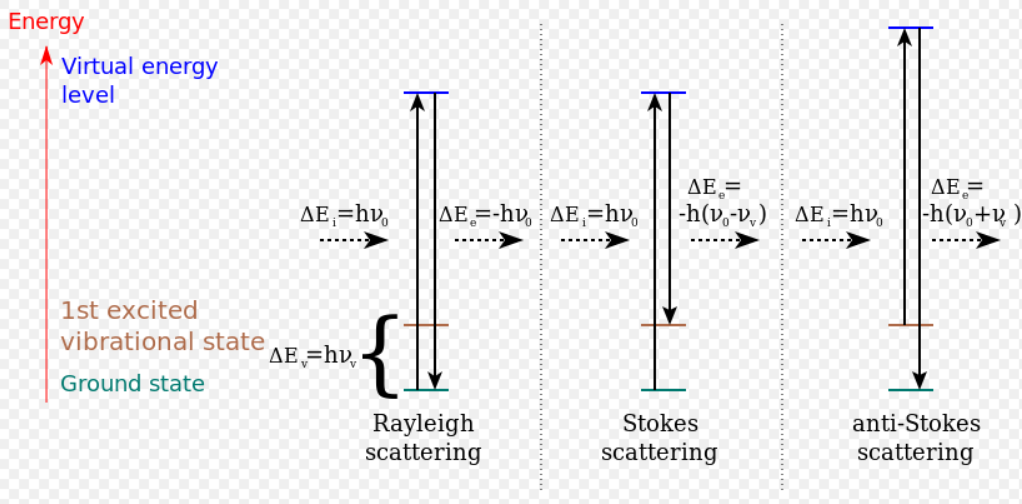
\includegraphics[width=1\linewidth]{Rozpraszanie-Ramanowskie/Raman-Energy.png}
		\caption{Diagram energetyczny przejść dla poszczególnych rodzajów rozpraszania.}
	\end{center}
\end{figure}
Widmo antystokesowskie jest mniej intensywne niż widmo stokesowskie. To jest spowodowane tym, że prawdopodobieństwo oddziaływania fotonu z cząsteczką będącą w stanie wzbudzonym jest dużo mniej prawdopodobne niż z cząsteczką w stanie podstawowym.

\subsection{Czynniki warunkujące zaistnienie zjawiska Ramana}
\subsubsection{Idealny dipol}
Przykładem takiego dipola może być układ składający się ze stacjonarnego ładunku dodatniego $+Q$ i ładunku ujemnego $-Q$, harmonicznie oscylującego wzdłuż kierunku $\overrightarrow{P}$ z częstotliwością $\omega$.
\begin{equation}
	p = p_{0}\cos(\omega t)
\end{equation}
Problem promieniowania dipola ma istotne znaczenie w teorii układów emitujących promieniowanie, ponieważ każdy rzeczywisty układ emitujący (na przykład antena) może być obliczony na podstawie promieniowania dipola. Ponadto wiele pytań dotyczących interakcji promieniowania z materią można wyjaśnić na podstawie klasycznej teorii, biorąc pod uwagę atomy jako układy ładunków, w których elektrony wykonują oscylacje harmoniczne wokół pozycji równowagowej.

Jeśli fala rozchodzi się w jednorodnym ośrodku izotropowym, to czas dotarcia fali do punktów odległych od dipola o odległość $r$ jest taki sam. Dlatego we wszystkich punktach kuli, której środek pokrywa się z dipolem, faza oscylacji jest taka sama, to znaczy w strefie falowej czoło fali będzie sferyczne, a w konsekwencji fala emitowana przez dipol jest falą sferyczną.

W każdym punkcie przestrzeni wektory $\overrightarrow{E}$ i $\overrightarrow{H}$ oscylują zgodnie z zależnością $\cos(\omega t - kr)$ a amplitudy tych wektorów są proporcjonalne do
$\frac{\sin \theta}{r}$ (dla próżni). Z wzorów tych wynika, że zależą one od odległości $r$ od środka dipola i kąta $\theta$ między kierunkiem momentu dipolowego i kierunkiem obserwacji.
\begin{figure}[H]
	\begin{center}
		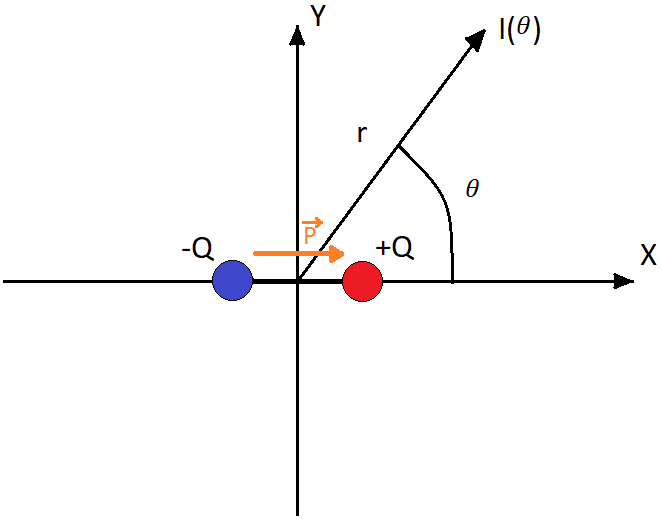
\includegraphics[width=0.6\linewidth]{Rozpraszanie-Ramanowskie/Point-Dipol.png}
		\caption{Drgający dipol, który tworzą dwa ładunki $-Q$ i $+Q$. $I(\theta)$ jest natężeniem promieniowania w odległości $r$ obserwowanym pod kątem $\theta$.}
	\end{center}
\end{figure}
Wynika stąd, że natężenie promieniowania dipolowego wynosi:
\begin{equation}
	I \sim \frac{\sin^{2}\theta}{r^{2}}
\end{equation}
Dla $\theta = \frac{\pi}{2}$ intensywność promieniowania jest maksymalna, a dla 
$\theta = 0$ i $\theta = \pi$ jest minimalna i wynosi $0$. Czyli dipol nie promieniuje wzdłuż kierunku momentu dipolowego.
\subsubsection{Realny dipol}
Warunkiem zaistnienia zjawiska Ramana są zmiany polaryzowalności cząsteczki w trakcie danego drgania. Polaryzowalność jest wielkością, którą można wyrazić za pomocą tensora drugiego rzędu, który jest macierzą 3x3 składającą się z 9 współczynników:
\begin{equation}
	\alpha = 
	\begin{bmatrix}
	\alpha_{xx} & \alpha_{xy} & \alpha_{xz} \\
	\alpha_{yx} & \alpha_{yy} & \alpha_{yz} \\
	\alpha_{zx} & \alpha_{zy} & \alpha_{zz}
	\end{bmatrix}
\end{equation}
Gdy mówimy np. o indukowanym momencie dipolowym, to pierwszy index współczynników oznacza kierunek momentu dipolowego, a drugi -- kierunek przyłożonego zewnętrznego pola elektrycznego.

\newpage
\subsection{Przykładowe widma ramanowskie}
Przykładowe widma ramanowskie dla materiałów $\mathbf{GaS}$ i $\mathbf{Ga_{2}S_{3}}$ zostało przedstawione na poniższym rysunku:
\begin{figure}[H]
	\begin{center}
		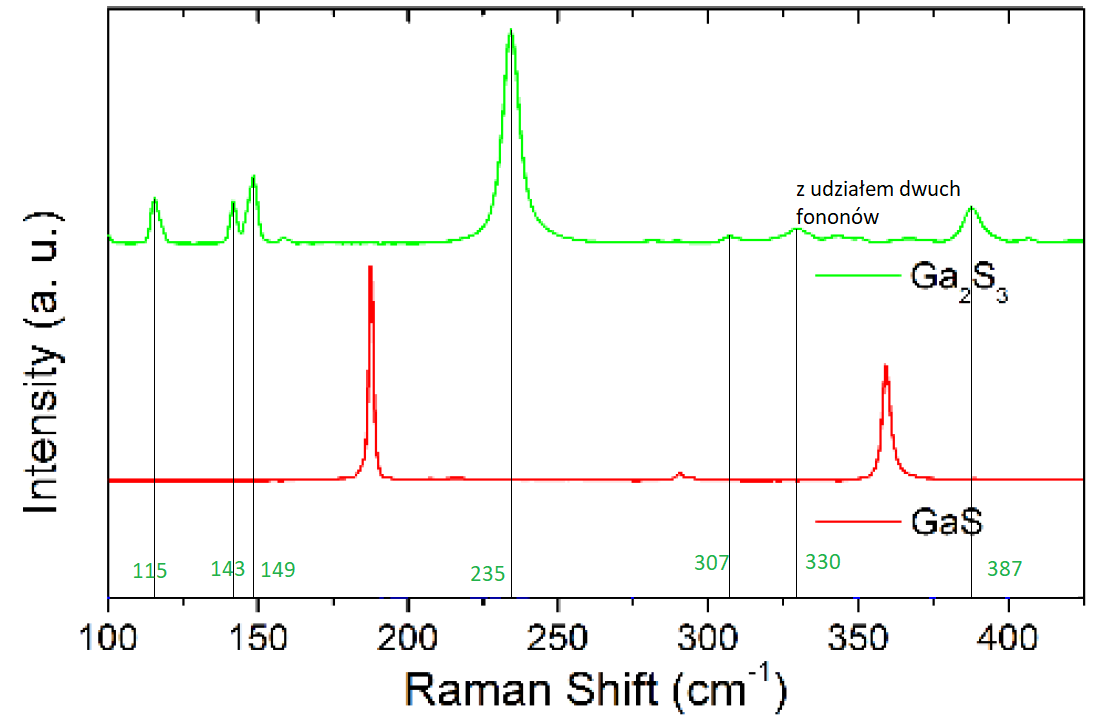
\includegraphics[width=0.8\linewidth]{Rozpraszanie-Ramanowskie/Raman-Shift.png}
		\caption{Widma rozpraszania ramanowskiego dla materiałów $GaS$ i $Ga_{2}S_{3}$ [25].}
	\end{center}
\end{figure}
Na powyższym rysunku pokazana jest tylko część stokesowska widma, ponieważ tylko tą częścią będę się zajmował w swojej pracy.

Energia fotonu wynosi:
\begin{equation}
	E = h \nu = h \frac{c}{\lambda} = hc \frac{1}{\lambda} 
\end{equation}
\begin{itemize}
	\item[-]{$h$ - stała Plancka};
	\item[-]{$c$ - prędkość światła};
	\item[-]{$\lambda$ - długość fali}.
\end{itemize}
Czyli odwrotność długości jest proporcjonalna do energii:
\begin{equation}
	\lambda^{-1} \sim E
\end{equation}

Zeru na powyższym widmie odpowiada energia światła pobudzającego (lasera). Wobec tego przesunięcie w widmie stokesowskim można zapisać w następując sposób:
\begin{equation}
	\frac{1}{\lambda} = \left| \frac{1}{\lambda_{Laser}} - \frac{1}{\lambda_{stok}} \right|
\end{equation}
\begin{itemize}
	\item[-]{$\lambda_{Laser}$ - długość fali promieniowania laserowego};
	\item[-]{$\lambda_{stok}$ - długość fali promieniowania ramanowskiego stokesowskiego}
\end{itemize}

Historycznie zostało przyjęte wyrażanie długości fali w jednostkach $cm$. Stąd 8 $cm^{-1}$ odpowiada około 1 $meV$ w skali energii.













